2012年のILSVRC優勝モデルで,図\ref{arch_alexnet}に示す構造を持つ \cite{paper_alexnet}.下記特徴を持つ.

\begin{itemize}
	\item Rectified Linear Units(ReLU)による非線形変換導入で勾配消失問題の解決と学習の高速化.
	\item Local Response Normalization (LRN)による正規化で学習の安定化と高速化.当時,Local Constrast Normalization(LCN)と比較してより適切な正規化法と主張していたが,後のVGG Netで効果が認められなかったことや,Batch Normalizationの登場により近年のモデルでは利用されていない.
	\item Overlapping poolingによるプーリング層でのオーバーラップにより過学習を提言.
	\item 全結合層のDropoutによる学習時のニューロン無効化によりモデルの汎化性能を向上.
	\item Momentum SGDによる最適化で学習を安定化.
	\item 重み減衰による正則化で過学習を抑制.
	\item 学習率減衰で学習の収束度を向上.
\end{itemize}

\begin{figure} [H]
	\begin{center}
		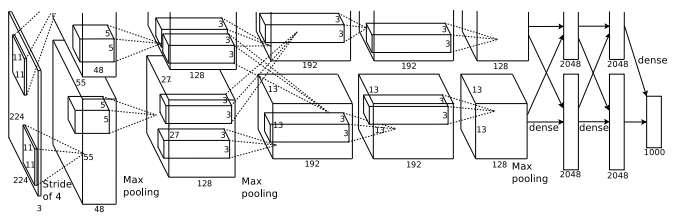
\includegraphics[clip, height=6cm, bb=-20 0 675 219]{data/figure/arch_alexnet.png}
		\caption{AlexNetアーキテクチャ}
		\label{arch_alexnet}
	\end{center}
\end{figure}
